\documentclass{article}

\usepackage{graphicx} % Required for the inclusion of images
\usepackage{natbib} % Required to change bibliography style to APA
\usepackage{amsmath} % Required for some math elements 

\setlength\parindent{0pt} % Removes all indentation from paragraphs

\renewcommand{\labelenumi}{\alph{enumi}.} % Make numbering in the enumerate environment by letter rather than number (e.g. section 6)

%\usepackage{times} % Uncomment to use the Times New Roman font
\usepackage{hyperref}
\usepackage{listings}
\usepackage{caption}
\usepackage{subcaption}


%----------------------------------------------------------------------------------------
%	DOCUMENT INFORMATION
%----------------------------------------------------------------------------------------
\title{Programming of Supercomputers \\ Final Report}
\author{Denys \textsc{Sobchyshak} and Denys \textsc{Korzh}}
\date{January 26, 2015}

\begin{document}
\maketitle

%----------------------------------------------------------------------------------------
%	SECTION 1
%----------------------------------------------------------------------------------------
\section{Introduction}
Programming of Supercomputers lab course deals to a great extent with a code that simulates flow and heat transfer within arbitrary complex geometries with fixed boundaries, also known as an AVL FIRE\textregistered\ benchmark. Most of the effort was focused on parallelizing and optimizing the benchmark code in order to prepare it for execution in multiprocessor environments. During the semester we had to complete the following tasks:
\begin{itemize}
	\item single-core optimization
	\item analysis of I/O behavior
	\item visualization
	\item 3-steps MPI parallelization
	\item performance tuning
\end{itemize}
In this report we will take a brief look at the summary of single-core optimization results and then move forward to parallelization aspects and their respective in depth analysis. It is important to note that all the measurements were carried out on a SuperMUC thin node.
%----------------------------------------------------------------------------------------
%	SECTION 2
%----------------------------------------------------------------------------------------
\section{Single-core optimization}
Quite often the great speedup potential of single-core execution of applications is overseen by many developers and instead all the effort is put into the parallelization step. This leads to inefficient usage of resources and poor scalability.
\\\\
This part of the course was focused solely on sequential optimization as a result of which we wanted to see how different optimization techniques relate to each other and what potential benefits our simulation code might obtain from them.
\\\\
The solver's execution was split into 3 main phases: input, computation and output. Analysis included collecting the following key characteristics for the computation phase using 2 input files (tjunc, cojack) and several optimization levels (-O1, -O2, -O3):
\begin{itemize}
	\item execution time
	\item Mflops
	\item L2 cache miss rate
	\item L3 cache miss rate
\end{itemize}
In addition we analysed the effect of vectorization on the computation phase using various compiler flags (-[no]-vec, -vec-report, -xhost).

\subsection{Performance measurements using PAPI}
In order to collect the measurements following hardware measurement counters of the Performance Application Programming Interface (PAPI) were used:\\
\begin{center}
\begin{tabular}{l|c}
	\hline
	Event & Description \\
	\hline
	PAPI\_DP\_OPS & Floating point operations; optimized to count vector operations \\
	PAPI\_L2\_TCM & Level 2 cache misses \\
	PAPI\_L2\_TCA & Level 2 total cache accesses \\
	PAPI\_L3\_TCM & Level 3 cache misses \\
	PAPI\_L3\_TCA & Level 3 total cache accesses \\
\end{tabular}
\end{center}
and consequently the next formulas to compute metrics were used:
\begin{center}
	$MFLOPS=\frac{PAPI\_FP\_OPS}{end\_time\_usec - start\_time\_usec}$
\end{center}
\begin{center}
	$L2\_CACHE\_MISS\_RATE=\frac{PAPI\_L2\_TCM}{PAPI\_L2\_TCA}*100$
\end{center}
\begin{center}
	$L3\_CACHE\_MISS\_RATE=\frac{PAPI\_L3\_TCM}{PAPI\_L3\_TCA}*100$
\end{center}
where end\_time\_usec and start\_time\_usec are corresponding PAPI start and end time values.

\subsubsection{Execution time}
With regard to execution time we observed that runtime of the computation phase decreased by roughly 23\% once the -O3 flag was utilized. Such aggressive loop optimization for speed can be seen on figure \ref{fig:1}.
\begin{figure}[h!]
	\begin{center}
		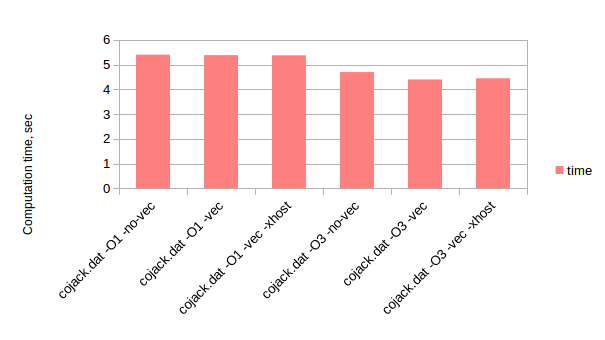
\includegraphics[width=0.8\textwidth]{comp-time}
		\caption{Comparison of computational time}
		\label{fig:1}
	\end{center}
\end{figure}

\subsubsection{Cache miss rates}
Usage of -O3 flag increased the cache miss rates for both L2 and L3 caches by a rough 22\%. Such effects of vectorisation on cache miss rates can be seen on figure \ref{fig:2}.
\begin{figure}[h!]
	\begin{center}
		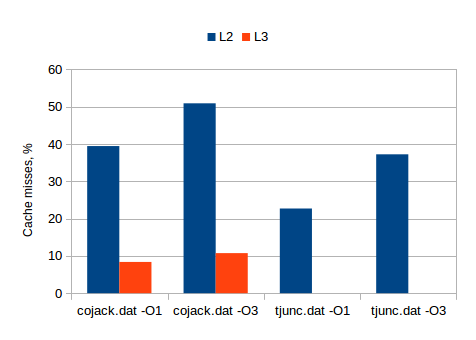
\includegraphics[width=0.8\textwidth]{cache-misses}
		\caption{Comparison of cache misses}
		\label{fig:2}
	\end{center}
\end{figure}

\subsubsection{MFLOPS counters}
We observed that once -O3 flag was employed measured MLUPS increased only marginally, analysis of such a delicate matter is hard to perform with raw instruments, however it is known that optimization might include various techniques like excluding common calculations out of loops, pre-calculating expressions, fusing constants and so on which will decrease the number of operations performed while the actual runtime might not decrease substantially.

\subsubsection{Effect of vectorization}
While carrying out measurements of vectorized versus novectorised benchmark runtime under different optimization options we have observed that enabled vectorization versus disabled one decreases the runtime of simulation by roughly 7\%. Furthermore, we measured computation time while having -xhost flag enabled and it slows down the simulation by around 1.2\%. This is most likely observed because vectorization can sometimes slow execution due to pipeline synchronization, data movement timing or other issues.

%----------------------------------------------------------------------------------------
%	SECTION 3
%----------------------------------------------------------------------------------------
\subsection{I/O performance analysis}
Manipulating data files is very slow compared to accessing the main memory. This can be considerably improved by using a more concise data format such as binary. After comparing input file sizes and the time it takes to load them we have noticed a drastic fall in both processing time and binary file sizes. Visualized comparison of loading times and file sizes is shown on figure \ref{fig:3}.

\begin{figure}[h!]
	\begin{center}
		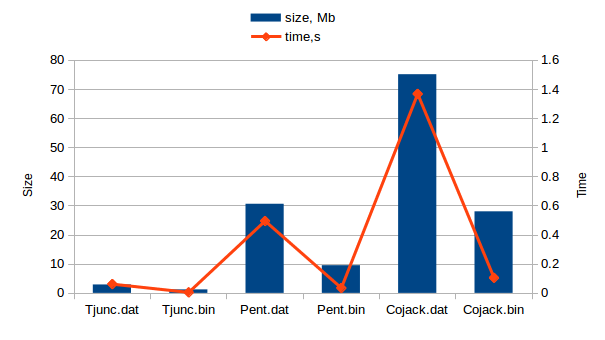
\includegraphics[width=0.8\textwidth]{time-size}
		\caption{Comparison of file sizes and their read times}
		\label{fig:3}
	\end{center}
\end{figure}
%----------------------------------------------------------------------------------------
%	SECTION 4
%----------------------------------------------------------------------------------------
\section{MPI parallelization}
The goal of entire parallelization part was to generate a parallel optimal version of the Fire benchmark which would scale in a multi-core environment.

\subsection{Data distribution}
We started off with an implementation of a computation domain and initial data distribution with focus on two types of data partitioning, namely:
\begin{itemize}
	\item classic distribution
	\item METIS distributions (nodal and dual)
\end{itemize}

\subsubsection{Classical distribution}
The core principle of this distribution was to separate all cells almost equally among available processors. Thus volume cells are partitioned in the order given by the input file: first k cells to the first process, next k cells to the second one, and so on. Such approach does not consider special location of the cells and thus the resulting partition map looks slightly random and very mixed as can be seen from figure \ref{fig:4}
\begin{figure}[h!]
	\begin{center}
		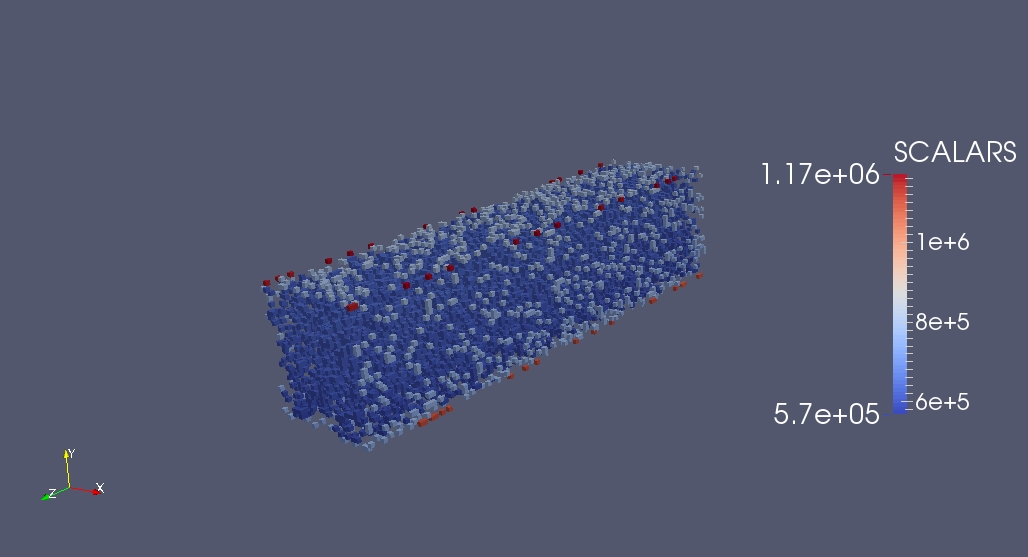
\includegraphics[width=0.8\textwidth]{pent-classic.jpg}
		\caption{Cells of single partition in a classic distribution model}
		\label{fig:4}
	\end{center}
\end{figure}
Key issue in this part was to figure out how our geometry looks and how we can work with it, thus understand binary file format and its content. The biggest role in this process played the following arrays:
\begin{itemize}
	\item[lcc] - link cell-to-cell array, which stores cell topology
	\item[elems] - IDs of nodes that form a cell
	\item[points] - coordinates of nodes
\end{itemize}

\subsubsection{METIS partitioning}
The latter data distribution strategy employed a special graph partitioning library METIS where we utilized two different distributions:
\begin{itemize}
	\item dual (METIS PartMeshDual) - partitions a mesh into k parts based on a partitioning of the mesh’s dual graph (i.e., each element becomes a graph vertex)
	\item nodal (METIS PartMeshNodal) - partitions a mesh into k parts based on a partitioning of the mesh’s nodal graph (i.e., each node becomes a graph vertex)
\end{itemize}
Examples of the partitioned data visualisation can be found on figure \ref{fig:5} along with a partition matrix on figure \ref{fig:15}.
\begin{figure}
	\centering
	\begin{subfigure}[b]{0.45\textwidth}
		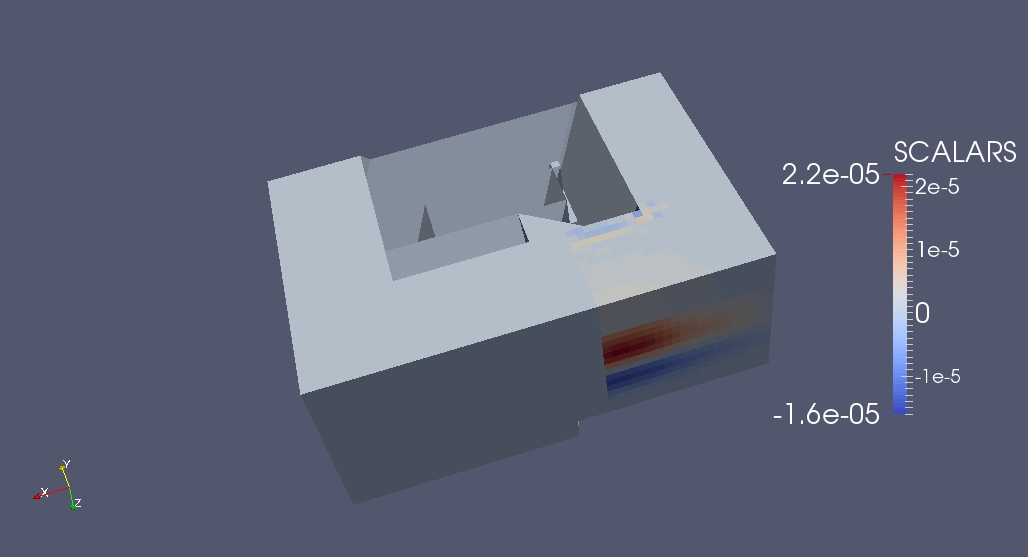
\includegraphics[width=\textwidth]{drall-dual.jpg}
		\caption{Dual partitioning of drall data}
		\label{fig:dual}
	\end{subfigure}%
	\begin{subfigure}[b]{0.45\textwidth}
		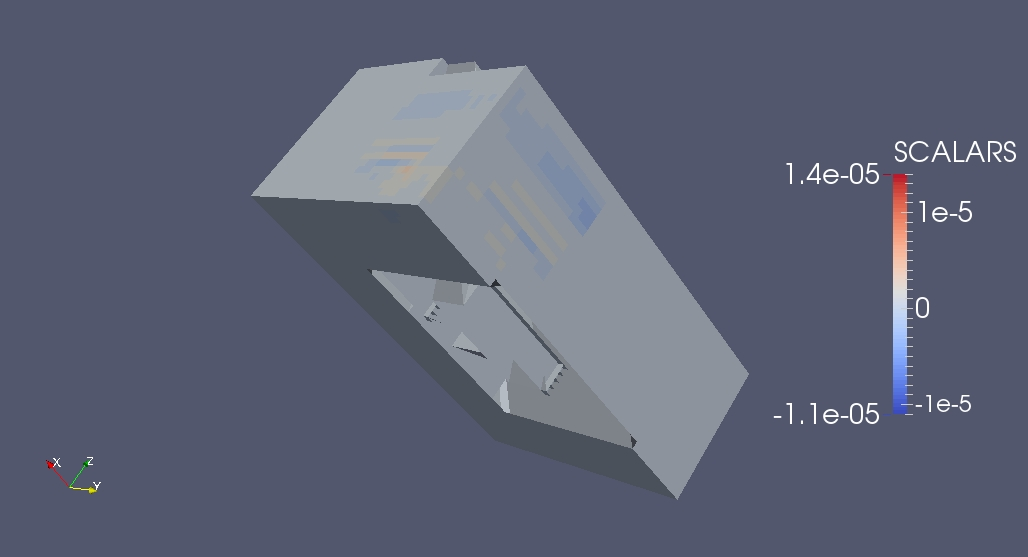
\includegraphics[width=\textwidth]{drall-nodal.jpg}
		\caption{Nodal partitioning of drall data}
		\label{fig:nodal}
	\end{subfigure}
	\caption{METIS data distribution visualisation}\label{fig:5}
\end{figure}

\begin{figure}
	\centering
	\begin{subfigure}[b]{0.45\textwidth}
		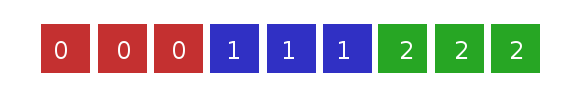
\includegraphics[width=\textwidth]{rectangles-classic.png}
		\caption{Schematic representation of classic partition map}
		\label{fig:class}
	\end{subfigure}%
	\begin{subfigure}[b]{0.45\textwidth}
		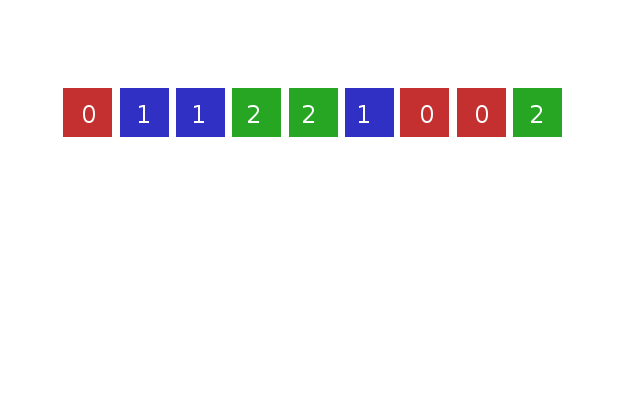
\includegraphics[width=\textwidth]{rectangles-metis.png}
		\caption{Schematic representation of metis partition map}
		\label{fig:metis}
	\end{subfigure}
	\caption{Classic vs METIS partitioning map schematic representation}\label{fig:15}
\end{figure}


\subsubsection{Data reading strategies}
One of the key issues of the first milestone was concerned with data reading strategy. It was crucial since some of the binary files would be as big as 45MB. We had two options to consider:
\begin{itemize}
	\item \textit{Oneread} - only one processor reads the data and communicates it among others
	\item \textit{Allread} - reading data on each processor
\end{itemize}
While \textit{oneread} strategy was rather straightforward and involved only proper MPI implementation, \textit{allread} strategy could be done in several ways. 
\begin{enumerate}
	\item One could read geometry data in each process, then individually perform data partitioning using either classic or METIS approaches and, assuming that data distribution is a deterministic operation (for same geometry partitioning will always stay the same), simply proceed with reading required values (bs, be, etc arrays) and performing the computation.
	\item Alternatively, each process could still read basic geometry data, then perform partitioning only on one process and communicate it to other processes, after which those processes would read necessary values (bs, be, etc arrays) and start the computation.
\end{enumerate}
We decided to stick with the first option leaving analysis of the latter one for the last milestone and as it turned out former approach was much more performant, since no process had to wait for another in order to continue with computations. Also the latter approach would add up to MPI communication overhead which is another unwanted drawback.

\subsection{Communication model}
At this point we would already have read and distributed data for further computation, however, to perform the computation on any cell we require values of all its neighbours. For inner cells of the partition it is easy to do, since all of them reside in the local memory of the current execution core, however, for cells with neighbours in other cores (ghost cells) things become a bit tricky.
\\\\
To tackle this problem we created send and receive lists for all neighbours of each process which would hold indexes of cells to be exchanged with the corresponding neighbour. We performed two cycles of inner cell processing in order to create send and receive counters first (send\_cnt and recv\_cnt) and then perform memory allocation and actual array filling. Our send and receive lists are 2D arrays where their 1st dimension corresponds to neighbor partition and 2nd dimension - to the local index of a ghost cell. Visualisation of send lists is provided in figure \ref{fig:6}
\begin{figure}[h!]
	\begin{center}
		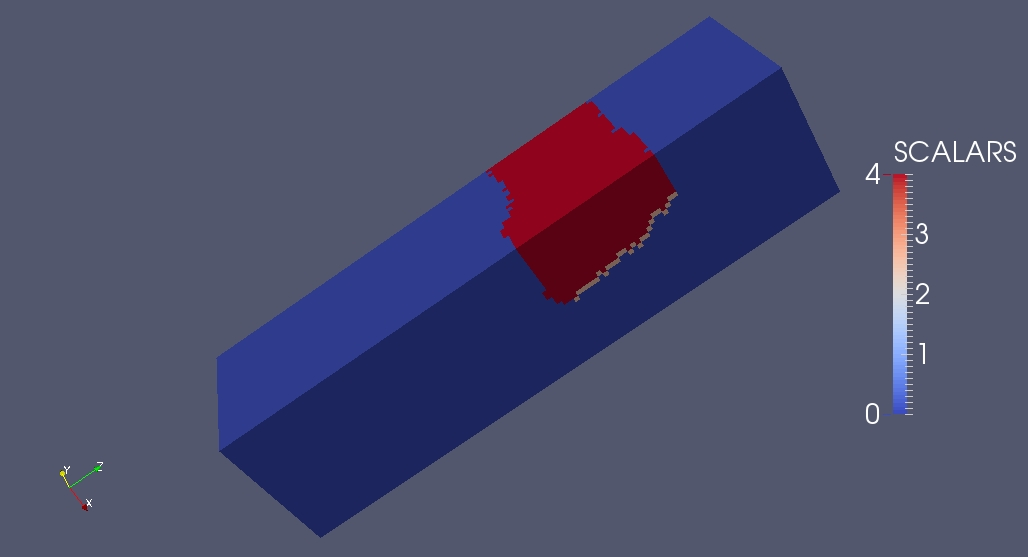
\includegraphics[width=0.8\textwidth]{send-listst.jpg}
		\caption{Inner cells and send lists}
		\label{fig:6}
	\end{center}
\end{figure}
\\\\
The fact that cells might have common ghost neighbours was also taken into account, so repeating indices of the receive list were not added to the array.
\\\\
As a side note, all of the global-to-local mappings were achieved using various mapping arrays, like \textit{nghb\_to\_rank}, \textit{g2l}, \textit{l2g}, etc.

\subsubsection{Non-Blocking communications}
In such a communication matrix where we don't have constant control over the number of processes (since the code could be run with 8, 256 or more processes) and order of data exchange - dead locks may become a threat. To avoid this issue and to increase performance of our code we used non-blocking MPI operations where possible.

\subsection{Main loop parallelization}
As a final prallelisation step, we needed to adjust computation phase to utilize MPI calls. As \textit{direc} vectors store the current solution state in the main loop, computing the cell value of the \textit{direc2} vector requires access to \textit{direc1} values of the cell’s neighbours, which might be outside of the local domain. For that purpose we need to use MPI non-blocking exchange functions and our previously filled send and receive lists. Now we know how many elements are to be received and from which processes.
\\\\
Earlier in the lab we discovered that usage of an MPI Indexed Data Type is advantageous in situations when we don't want to create small buffers in order to exchange parts of a big array. We took full advantage of the approach here as well, using \textit{MPI\_Type\_indexed}.

\section{Performance tuning}
The final step of the benchmark parallelisation and optimization focused on code tuning. Minimum requirement was to achieve \textit{linear speedup} of the computation phase up to 8 processes for \textit{pent} input geometry using the \textit{dual} distribution. Apparently, due to proper coding styles and also due to the fact that we didn't start working on the performance analysis code untill most of our TODOs (planned tasks) were resolved, already from the start we had linear speedup depicted on figure \ref{fig:11}. Also we had rather low MPI overhead (excluding \textit{MPI\_Init} and \textit{MPI\_Finalize}) as shown on the figure \ref{fig:12}. However, we still performed recommended performance analysis and couple of optimizations described further.
\begin{figure}[h!]
	\begin{center}
		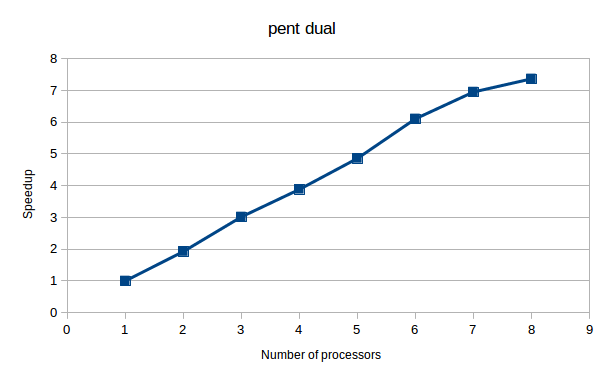
\includegraphics[width=0.8\textwidth]{pent_computation_speedup_1-8proc.png}
		\caption{Base code speedup}
		\label{fig:11}
	\end{center}
\end{figure}
\begin{figure}[h!]
	\begin{center}
		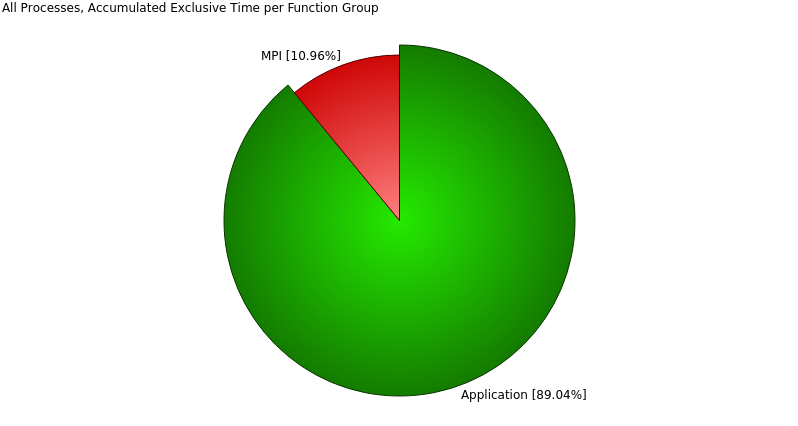
\includegraphics[width=0.8\textwidth]{no_mpi_init_finalize-pent-dual-allread-8-Function_Summary_traces.png}
		\caption{MPI overhead for pent dual allread on 8 processors}
		\label{fig:12}
	\end{center}
\end{figure}

\subsection{Mesurements}
Before we dig into the optimizations and performance analysis it is useful to describe our time measurement approach and some of the tools we have created for metric collection. 

\subparagraph{Timing}
Since we needed to optimize only specific parts of the application and not the total runtime, we explicitly blocked all MPI operations between application phases (initialization, computation, finalization) using \textit{MPI\_Barrier}. This made time measurement using \textit{MPI\_Wtime} extremely easy since we didn't have to worry if all processes arrived to the Wtime call at approximately same time or if some of the processes were still stuck in the previous phase. We used \textit{MPI\_Reduce} to collect global minimum and maximum times for the specified phase and so obtained the actual time measurement of each application phase.

\subparagraph{Bash framework}
Furthermore, since we had to perform numerous measurements with different number of processors and various codes (optimized and non-optimized versions), we decided to create a small bash framework: our script would receive number of processors and an optimization identifier (e.g. \textit{optimization2}) after which it would automatically generate proper job files (with correct number of nodes and etc.), submit them, wait for the jobs to complete and then combine all the outputs into one file and errors into another. In such a way the whole process of job submission and data collections was significantly simplified.

\subsection{Analysis tools}

\subparagraph{Score-P}
For a proper code analysis we used Score-P performance measurement infrastructure - a highly scalable and easy-to-use tool suite for profiling, event tracing, and online analysis of HPC applications. It can be controlled via environment variables and is as easy to set up as to just add it to the makefile. Next run of the application will create Score-P analysis files in the previously specified directories. After that one has to use specific tools to visualise the output and investigate bottlenecks.

\subparagraph{Cube}
A tool used for viewing and analyzing profile data, which is useful to take down big bottlenecks. 

\subparagraph{Vampir}
Tool used for investigation of trace information, which is useful for in-depth MPI overhead analysis. It also allowed to identify low FLOPS regions in our code as in figure \ref{fig:7}.
\begin{figure}[h!]
	\begin{center}
		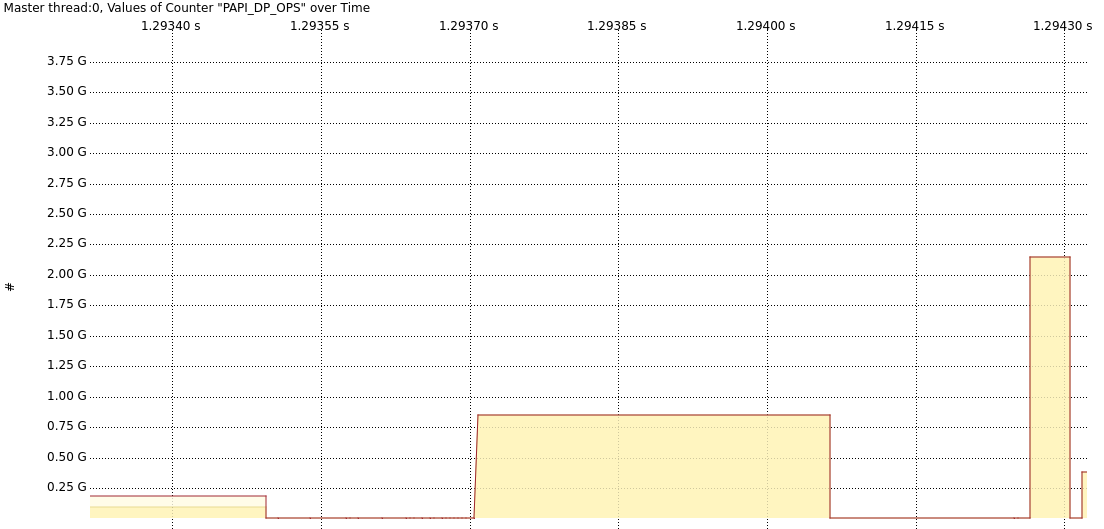
\includegraphics[width=0.8\textwidth]{iter-pent-dual-allread-8-Counter_Data_Timeline_traces.png}
		\caption{Regions with low FLOPS}		
		\label{fig:7}
	\end{center}
\end{figure}

\subparagraph{TotalView}
Is a set of tools which provide unprecedented control over processes and thread execution, along with deep visibility into program states and data, which was of great use for per processor debugging. However, on SuperMUC we could use it only with intel compiler.

\subsection{File reading optimization}
One of the early things we noticed using Cube is that sometimes initialization phase would take even more time than the actual computation phase. After some investigation we came with an idea of reading only specific data from our input files, since those can be as big as 45Mb reading everything on all processors takes too much time. Achieved performance can be seen on figure \ref{fig:13} as compared to the original one. It affected the fastest input data processing strategy \textit{allread} thus potentially decreasing runtime of the whole application.
\begin{figure}[h!]
	\begin{center}
		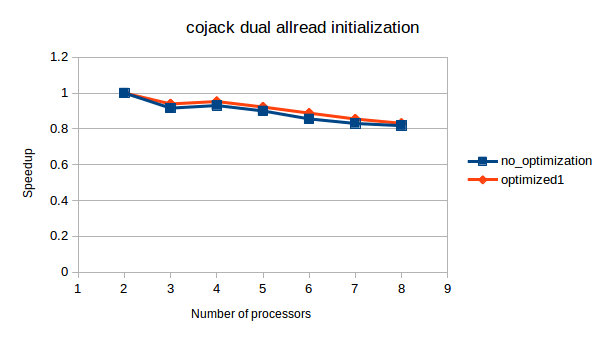
\includegraphics[width=0.8\textwidth]{cojack_inputalgorithm_scalability.png}
		\caption{Scalability of cojack input data processing (higher is better)}
		\label{fig:13}
	\end{center}
\end{figure}

\subsection{MPI data type optimization}
Analysing Vampir timeline tracer we noticed that two very close MPI calls which don't have much computation in between were actually separated by a big block of computation. Analysing that block we noticed that much of its time was spent on allocating memory for \textit{MPI\_Type\_indexed} block length arrays and filling in the correct values. Since those operations take too much space and our block length actually never changes, we switched to using \textit{MPI\_Type\_create\_indexed\_block} which gave us a minor improvement. Vampire visualisation for the computation phase can be found in the figure \ref{fig:8}.
\begin{figure}
	\centering
	\begin{subfigure}[b]{\textwidth}
		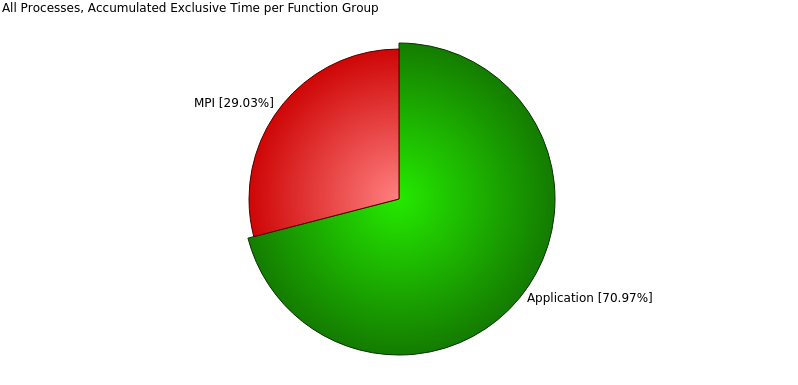
\includegraphics[width=\textwidth]{iter-pent-dual-allread-8-Function_Summary_traces.png}
		\caption{MPI Overhead}
		\label{fig:overhead}
	\end{subfigure}
	\begin{subfigure}[b]{\textwidth}
		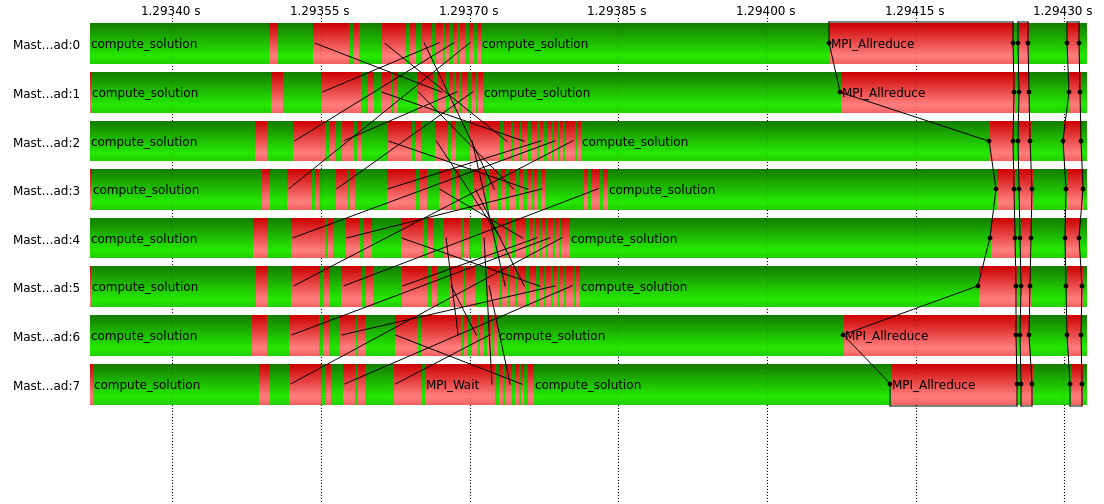
\includegraphics[width=\textwidth]{iter-pent-dual-allread-8-Master_Timeline_traces.png}
		\caption{Timeline traces}
		\label{fig:traces}
	\end{subfigure}
	\begin{subfigure}[b]{\textwidth}
		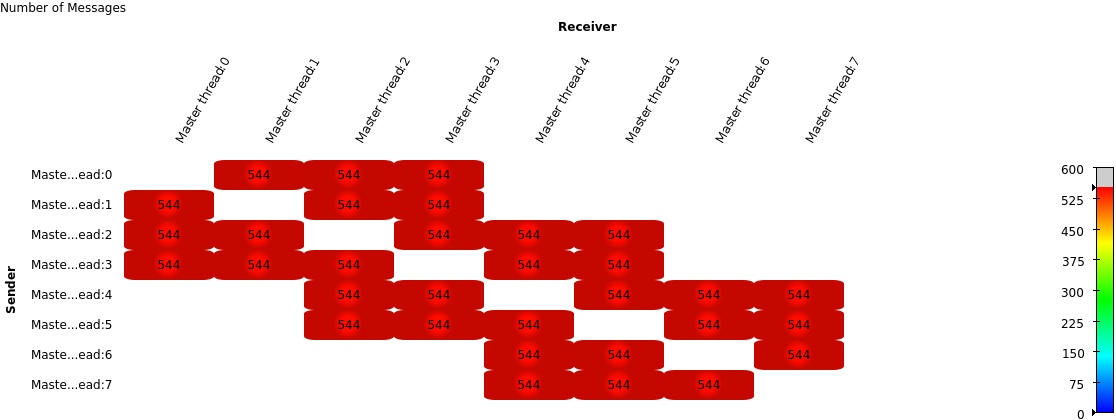
\includegraphics[width=\textwidth]{comp-pent-dual-allread-8-Communication_Matrix_View_traces.png}
		\caption{Communication matrix}
		\label{fig:commatrx}
	\end{subfigure}
	\caption{Computation phase trace timeline}\label{fig:8}
\end{figure}

\subsection{Memory leaks}
While using TotalView we noticed a lot of memory leaks in our code and also to a lesser extent in the provided benchmark. All of those were fixed and merged into the final version of the code.

%----------------------------------------------------------------------------------------
\end{document}